%!TeX encoding = UTF-8
%!TeX program = xelatex
\documentclass[notheorems, aspectratio=1610]{beamer}
% aspectratio: 1610, 149, 54, 43(default), 32

\usepackage{latexsym}
\usepackage{amsmath,amssymb}
\usepackage{mathtools}
\usepackage{color,xcolor}
\usepackage{graphicx}
\usepackage{algorithm}
\usepackage{amsthm}
\usepackage{lmodern}
\usepackage{animate} % insert gif
\usepackage{lipsum} % To generate test text
\usepackage{ulem}
\usepackage{listings} % display code on slides; don't forget [fragile] option after \begin{frame}

% ----------------------------------------------
% tikx
\usepackage{framed}
\usepackage{tikz}
\usepackage{pgf}
\usetikzlibrary{calc,trees,positioning,arrows,chains,shapes.geometric,%
    decorations.pathreplacing,decorations.pathmorphing,shapes,%
    matrix,shapes.symbols}
\pgfmathsetseed{1} % To have predictable results
% Define a background layer, in which the parchment shape is drawn
\pgfdeclarelayer{background}
\pgfsetlayers{background,main}

% define styles for the normal border and the torn border
\tikzset{
  normal border/.style={orange!30!black!10, decorate,
     decoration={random steps, segment length=2.5cm, amplitude=.7mm}},
  torn border/.style={orange!30!black!5, decorate,
     decoration={random steps, segment length=.5cm, amplitude=1.7mm}}}

% Macro to draw the shape behind the text, when it fits completly in the
% page
\def\parchmentframe#1{
\tikz{
  \node[inner sep=2em] (A) {#1};  % Draw the text of the node
  \begin{pgfonlayer}{background}  % Draw the shape behind
  \fill[normal border]
        (A.south east) -- (A.south west) --
        (A.north west) -- (A.north east) -- cycle;
  \end{pgfonlayer}}}

% Macro to draw the shape, when the text will continue in next page
\def\parchmentframetop#1{
\tikz{
  \node[inner sep=2em] (A) {#1};    % Draw the text of the node
  \begin{pgfonlayer}{background}
  \fill[normal border]              % Draw the ``complete shape'' behind
        (A.south east) -- (A.south west) --
        (A.north west) -- (A.north east) -- cycle;
  \fill[torn border]                % Add the torn lower border
        ($(A.south east)-(0,.2)$) -- ($(A.south west)-(0,.2)$) --
        ($(A.south west)+(0,.2)$) -- ($(A.south east)+(0,.2)$) -- cycle;
  \end{pgfonlayer}}}

% Macro to draw the shape, when the text continues from previous page
\def\parchmentframebottom#1{
\tikz{
  \node[inner sep=2em] (A) {#1};   % Draw the text of the node
  \begin{pgfonlayer}{background}
  \fill[normal border]             % Draw the ``complete shape'' behind
        (A.south east) -- (A.south west) --
        (A.north west) -- (A.north east) -- cycle;
  \fill[torn border]               % Add the torn upper border
        ($(A.north east)-(0,.2)$) -- ($(A.north west)-(0,.2)$) --
        ($(A.north west)+(0,.2)$) -- ($(A.north east)+(0,.2)$) -- cycle;
  \end{pgfonlayer}}}

% Macro to draw the shape, when both the text continues from previous page
% and it will continue in next page
\def\parchmentframemiddle#1{
\tikz{
  \node[inner sep=2em] (A) {#1};   % Draw the text of the node
  \begin{pgfonlayer}{background}
  \fill[normal border]             % Draw the ``complete shape'' behind
        (A.south east) -- (A.south west) --
        (A.north west) -- (A.north east) -- cycle;
  \fill[torn border]               % Add the torn lower border
        ($(A.south east)-(0,.2)$) -- ($(A.south west)-(0,.2)$) --
        ($(A.south west)+(0,.2)$) -- ($(A.south east)+(0,.2)$) -- cycle;
  \fill[torn border]               % Add the torn upper border
        ($(A.north east)-(0,.2)$) -- ($(A.north west)-(0,.2)$) --
        ($(A.north west)+(0,.2)$) -- ($(A.north east)+(0,.2)$) -- cycle;
  \end{pgfonlayer}}}

% Define the environment which puts the frame
% In this case, the environment also accepts an argument with an optional
% title (which defaults to ``Example'', which is typeset in a box overlaid
% on the top border
\newenvironment{parchment}[1][Example]{%
  \def\FrameCommand{\parchmentframe}%
  \def\FirstFrameCommand{\parchmentframetop}%
  \def\LastFrameCommand{\parchmentframebottom}%
  \def\MidFrameCommand{\parchmentframemiddle}%
  \vskip\baselineskip
  \MakeFramed {\FrameRestore}
  \noindent\tikz\node[inner sep=1ex, draw=black!20,fill=white,
          anchor=west, overlay] at (0em, 2em) {\sffamily#1};\par}%
{\endMakeFramed}

% ----------------------------------------------

\mode<presentation>{
    \usetheme{Luebeck}
    % Boadilla CambridgeUS
    % default Antibes Berlin Copenhagen
    % Madrid Montpelier Ilmenau Malmoe
    % Berkeley Singapore Warsaw
    \usecolortheme{beaver}
    % beetle, beaver, orchid, whale, dolphin
    \useoutertheme{infolines}
    % infolines miniframes shadow sidebar smoothbars smoothtree split tree
    \useinnertheme{circles}
    % circles, rectanges, rounded, inmargin
}
\setbeamercolor{block title}{bg=red!30,fg=white}

\newcommand{\reditem}[1]{\setbeamercolor{item}{fg=red}\item #1}

\newcommand*{\Scale}[2][4]{\scalebox{#1}{\ensuremath{#2}}}

\renewcommand\textbullet{\ensuremath{\bullet}}

% ---------------------------------------------------------------------
% flow chart
\tikzset{
    >=stealth',
    punktchain/.style={
        rectangle,
        rounded corners,
        % fill=black!10,
        draw=white, very thick,
        text width=6em,
        minimum height=2em,
        text centered,
        on chain
    },
    largepunktchain/.style={
        rectangle,
        rounded corners,
        draw=white, very thick,
        text width=10em,
        minimum height=2em,
        on chain
    },
    line/.style={draw, thick, <-},
    element/.style={
        tape,
        top color=white,
        bottom color=blue!50!black!60!,
        minimum width=6em,
        draw=blue!40!black!90, very thick,
        text width=6em,
        minimum height=2em,
        text centered,
        on chain
    },
    every join/.style={->, thick,shorten >=1pt},
    decoration={brace},
    tuborg/.style={decorate},
    tubnode/.style={midway, right=2pt},
    font={\fontsize{10pt}{12}\selectfont},
}
% ---------------------------------------------------------------------

% code setting
\lstset{
    language=C++,
    basicstyle=\ttfamily\footnotesize,
    keywordstyle=\color{red},
    breaklines=true,
    xleftmargin=2em,
    numbers=left,
    numberstyle=\color[RGB]{222,155,81},
    frame=leftline,
    tabsize=4,
    breakatwhitespace=false,
    showspaces=false,
    showstringspaces=false,
    showtabs=false,
    morekeywords={Str, Num, List},
}

% ---------------------------------------------------------------------

%% preamble
\title[Rings Slide Template]{PPT Template - Rings Slide Template}
% \subtitle{The subtitle}

\author[Rings Develop Team]{
  
\includegraphics[height=2cm]{./_temp/rings_rust.png}
  \\
  Rings Dev
}

%% preamble
\title[Rings 101]{Rings 101 - What is Distributed Network}
% \subtitle{The subtitle}

\author[Ryan Kung]{
  
\includegraphics[height=2cm]{../_temp/rings_rust.png}
  \\
  Ryan J. Kung
  \\
  Rings Network Dev Team
}

\begin{document}

%% title frame
\begin{frame}
    \titlepage
\end{frame}

\begin{frame}
  \frametitle{ What is Distributed Network }
  \begin{itemize}
  \item{ Definition: What is distributed system (1min) }
  \item{ Is internet distributed? (1min) }
  \item{ Intoduce to dWeb (1min) }
  \item{ Implementation of dWeb (1min) }
  \end{itemize}
\end{frame}

\begin{frame}
  \frametitle{ Definition: What is distributed system }
  \textbf{
  \LARGE
  A system is distributed if the message transmission delay is not negligible compared to the time between events in a single process. \cite{lamport1978}
  \begin{flushright}
   --- Leslie Lamport, 1978
  \end{flushright}
  }
  \note {
  In 1978, Leslie Lamport proposed this definition and made significant contributions to the field of distributed systems, for which he was awarded the Turing Award.
  }
\end{frame}


\begin{frame}
  \frametitle{Leslie Lamport at 1978 }
  \begin{figure}[h]
  \centering
  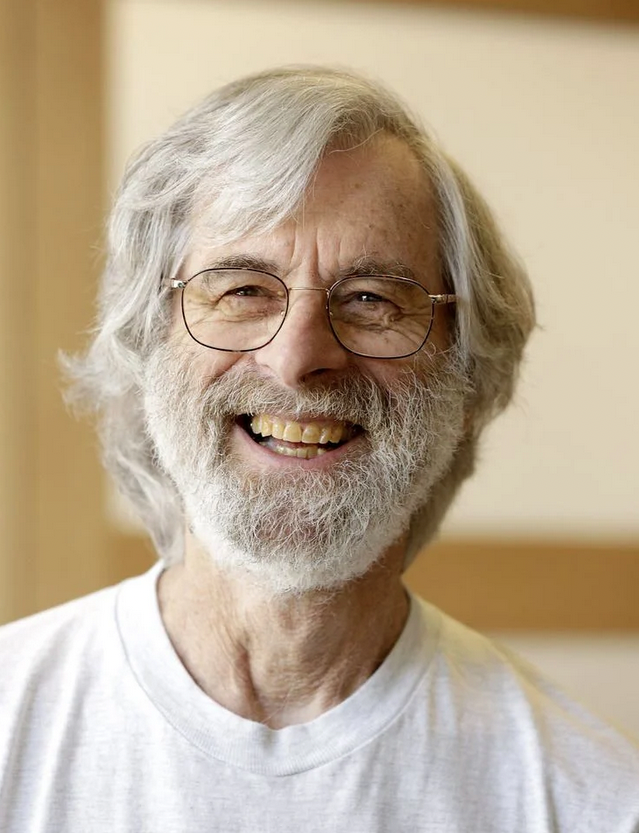
\includegraphics[height=0.4\linewidth]{lamport.png}
  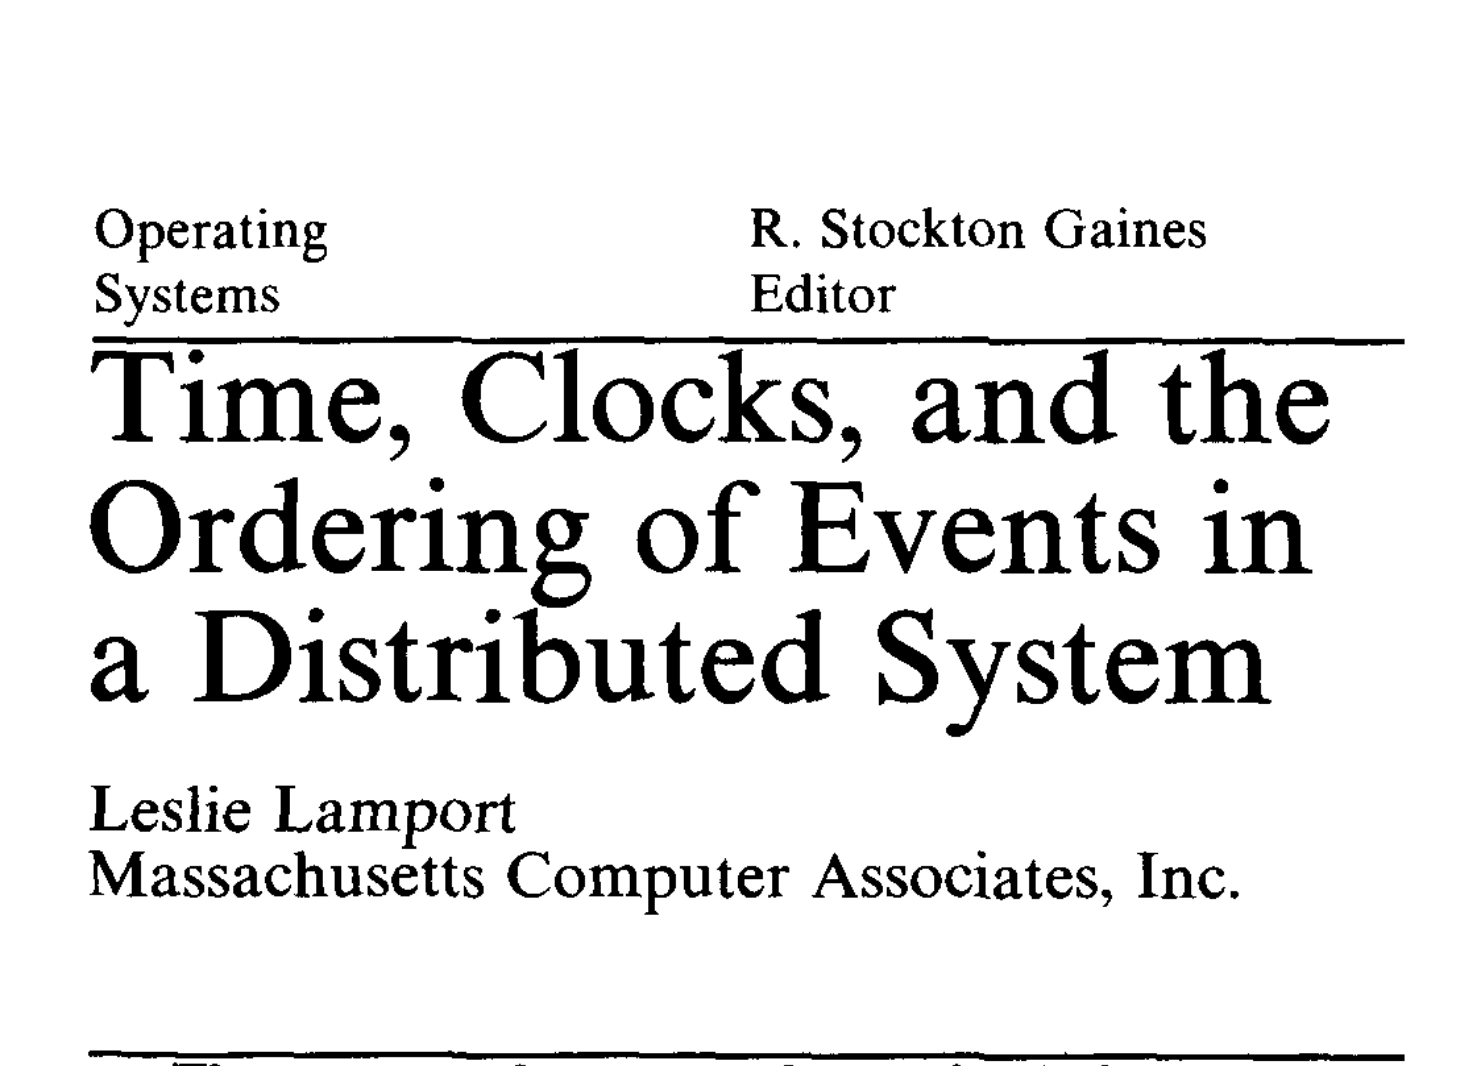
\includegraphics[width=0.5\linewidth]{lamport_paper.png}
  \end{figure}

  \note {
  In his classic paper titled "Time, Clocks, and the Ordering of Events in a Distributed System,"
  Lamport provided a description of distributed networks and introduced the "Lamport timestamp"
  as a mechanism for ordering events.
  In essence, Lamport invented logical time for the distributed world.
}
\end{frame}


\begin{frame}
  \frametitle{ Logical Timestamp }
  \begin{figure}[h]
  \centering
  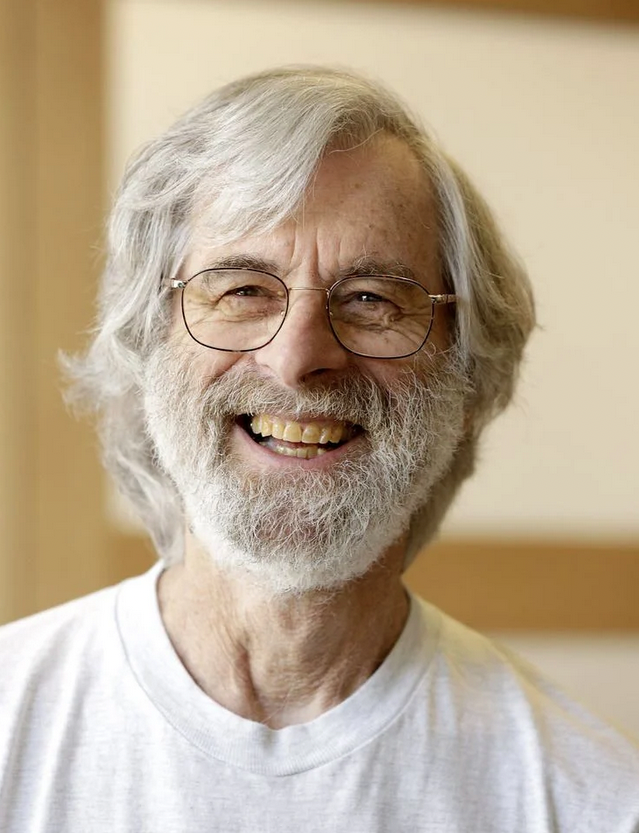
\includegraphics[height=0.4\linewidth]{lamport.png}
  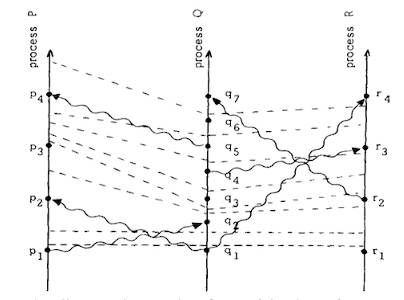
\includegraphics[width=0.5\linewidth]{lamport_timestamp.png}
  \end{figure}
  \note {
  The statement "message transmission delay is not negligible" in the definition of a distributed system hides an assumption that the delay in a distributed system is random and unpredictable. Therefore, given three peers A, B, and C, without any external information, C cannot independently determine the order of messages from A and B.

  The Lamport Timestamp provides a method for measuring time based on the ordering of messages, rather than relying on real-world time. This concept is extremely valuable, especially in complex distributed networks where message sequencing is essential. In the realm of cryptography, the sequencer holds paramount importance, particularly in Layer 2 implementations. We will delve deeper into this topic in future discussions.
}
\end{frame}

\begin{frame}
\frametitle{ Is Internet distributed? }
  \begin{figure}[h]
  \centering
  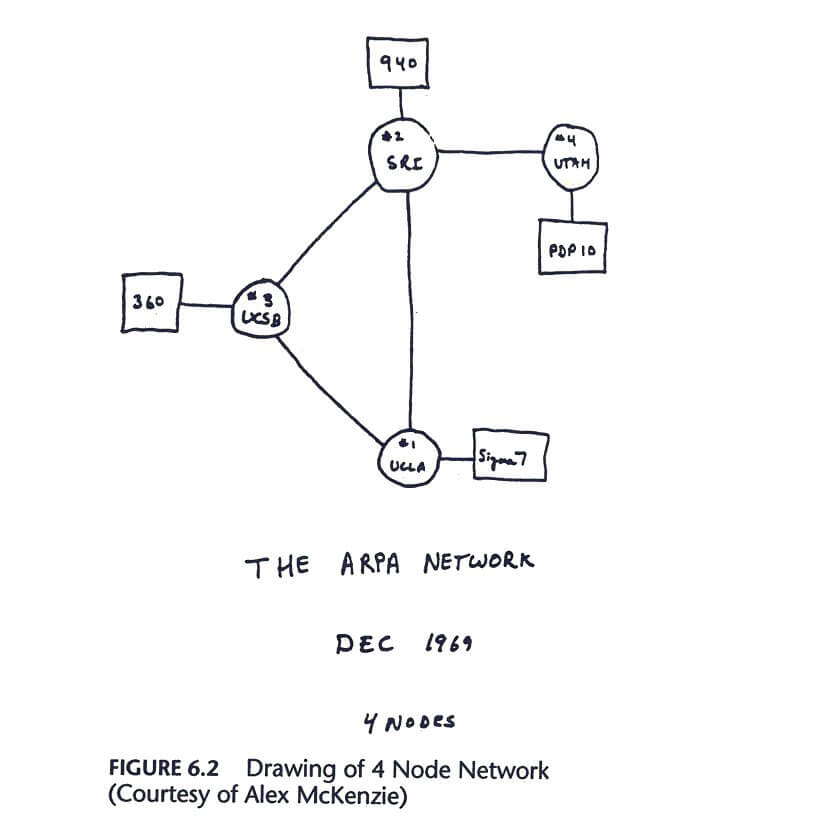
\includegraphics[height=0.5\linewidth]{arpa-1969.jpg}
  \end{figure}
\end{frame}

\begin{frame}
\frametitle{ Is Internet distributed? }
  \begin{figure}[h]
  \centering
  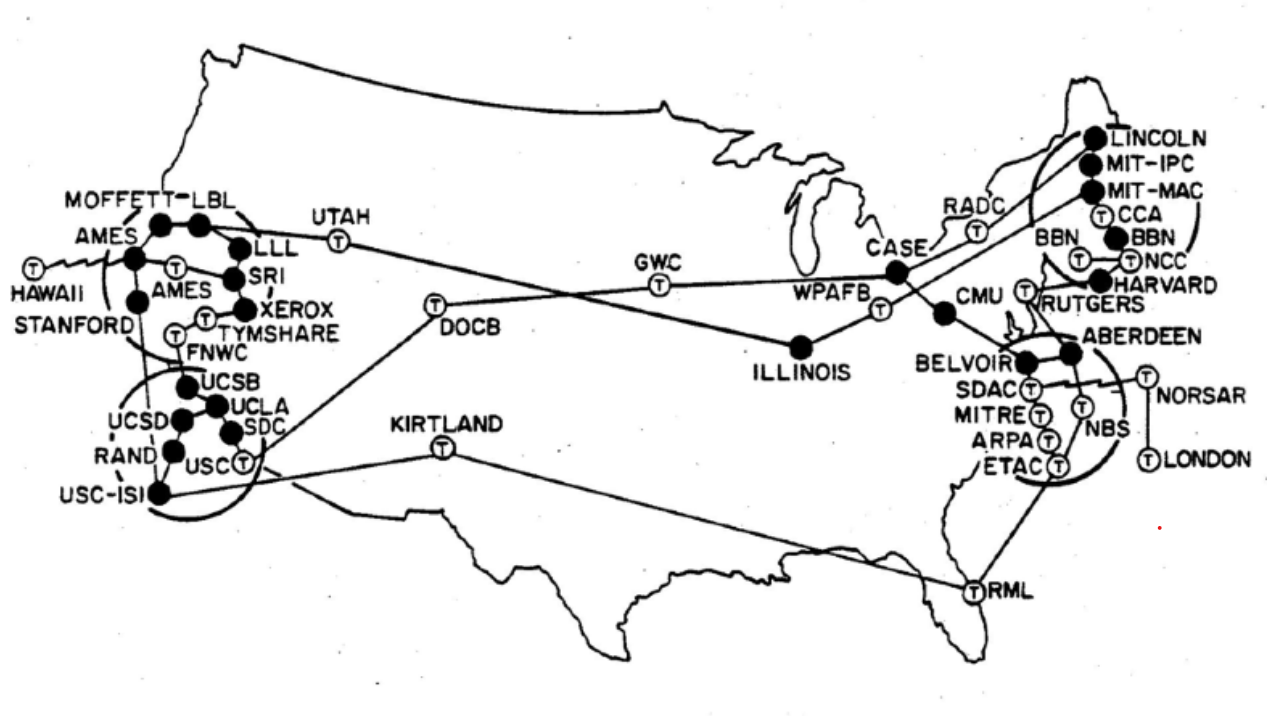
\includegraphics[height=0.5\linewidth]{arpa-1970.png}
  \end{figure}
\end{frame}

\begin{frame}
\frametitle{ Is Internet distributed? }
  \begin{figure}[h]
  \centering
  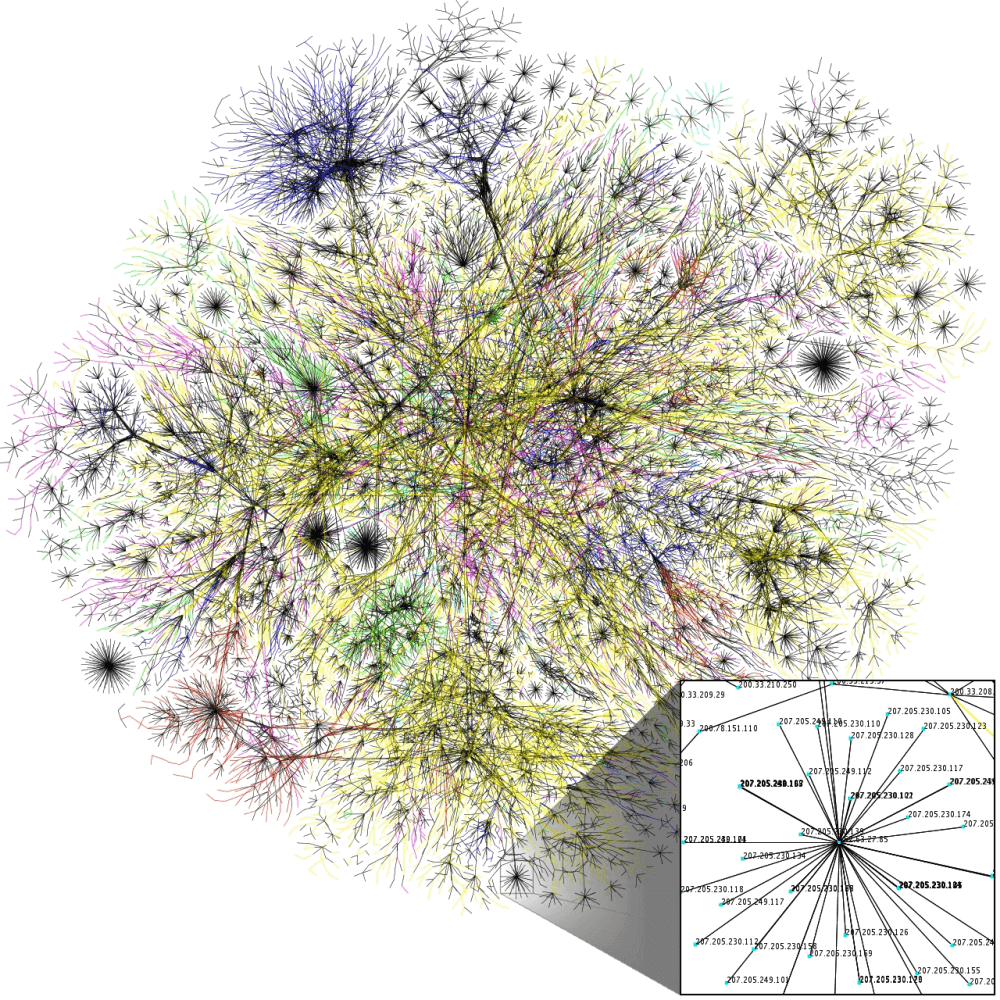
\includegraphics[height=0.5\linewidth]{web-img.png}
  \end{figure}
 \note {Visualisation of a possible routing path on the Internet. }
\end{frame}

\begin{frame}
\frametitle{ Centralized Internet }
\begin{columns}[T] % contents are top vertically aligned
\begin{column}{5cm} % each column can also be its own environment
  \begin{minipage}[c][0.5 \textheight][c]{\linewidth}
    \textbf{The system is failing.\cite{bernerslee2017}}
    \begin{flushright}
     --- Tim Berners-Lee, 2017
    \end{flushright}
  \end{minipage}
\end{column}
\begin{column}{5cm} % alternative top-align that's better for graphics
  \begin{figure}[h]
  \centering
  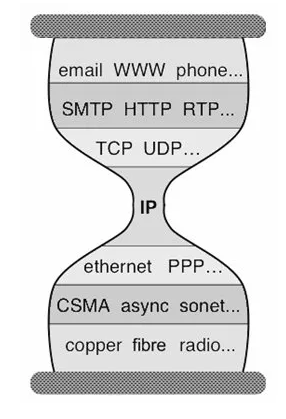
\includegraphics[width=0.7\linewidth]{hourglass.png}
  \end{figure}
\end{column}
\end{columns}
\end{frame}

\begin{frame}
\frametitle{ Centralized Internet }
  \begin{figure}[h]
  \centering
  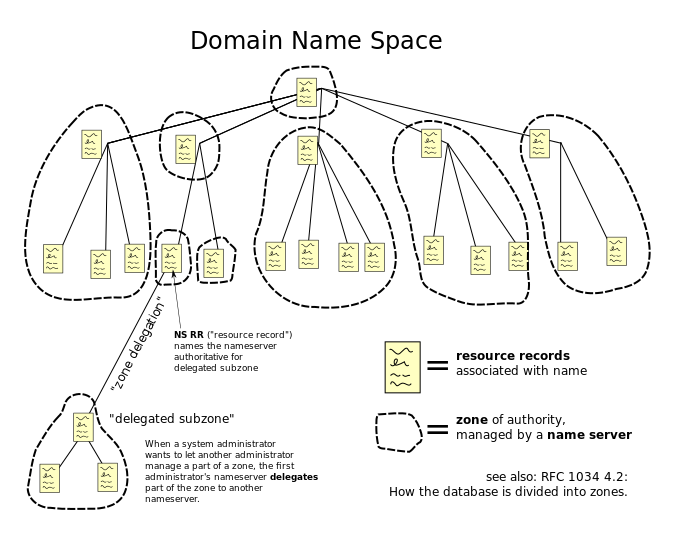
\includegraphics[height=0.5\linewidth]{dns.png}
  \end{figure}
\end{frame}


\begin{frame}
\frametitle{ Centralized Internet }
  \begin{figure}[h]
  \centering
  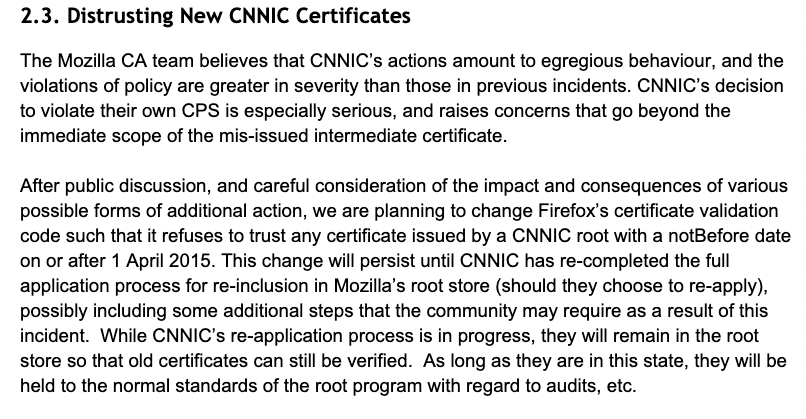
\includegraphics[height=0.4\linewidth]{CNNIC.png}
  \end{figure}
\end{frame}


\begin{frame}
\frametitle{ Intoducing to the dWeb }
  \begin{figure}[h]
  \centering
  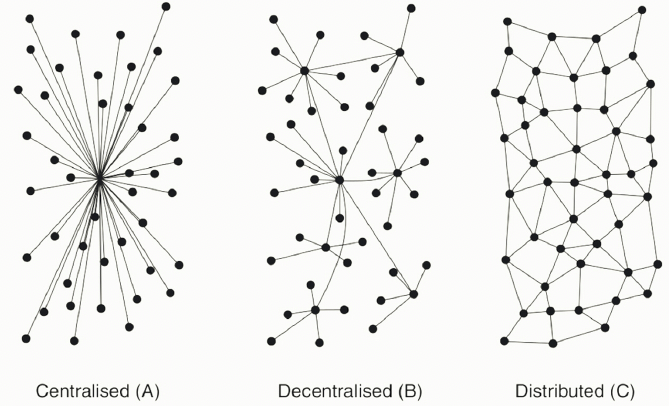
\includegraphics[width=0.7\linewidth]{lopologic.png}\cite{mozilla2018}
  \end{figure}
\end{frame}

\begin{frame}
\frametitle{ Implementation of dWeb }
  \begin{itemize}
  \item { Tor Project }
  - Onion Relay, Hidden services
  \item { GUNnet }
  - DHT Based, structure p2p
  \item { Rings Network }
  - DHT and WASM, structure p2p
  \end{itemize}
\end{frame}

\begin{frame}
  \frametitle{Thanks}
  Repository of this Slides:\newline \\
  \centering
  \color{black}{\fcolorbox{white}{white}{
  \qrcode[link, height=1in]{https://github.com/ringsnetwork/rings-101}
  }}
\end{frame}

\begin{frame}
    \frametitle{Reference}
  \bibliographystyle{plain}
  \bibliography{slide}
\end{frame}

\end{document}